% Options for packages loaded elsewhere
\PassOptionsToPackage{unicode}{hyperref}
\PassOptionsToPackage{hyphens}{url}
\PassOptionsToPackage{dvipsnames,svgnames,x11names}{xcolor}
%
\documentclass[
  letterpaper,
  DIV=11,
  numbers=noendperiod]{scrartcl}

\usepackage{amsmath,amssymb}
\usepackage{iftex}
\ifPDFTeX
  \usepackage[T1]{fontenc}
  \usepackage[utf8]{inputenc}
  \usepackage{textcomp} % provide euro and other symbols
\else % if luatex or xetex
  \usepackage{unicode-math}
  \defaultfontfeatures{Scale=MatchLowercase}
  \defaultfontfeatures[\rmfamily]{Ligatures=TeX,Scale=1}
\fi
\usepackage{lmodern}
\ifPDFTeX\else  
    % xetex/luatex font selection
\fi
% Use upquote if available, for straight quotes in verbatim environments
\IfFileExists{upquote.sty}{\usepackage{upquote}}{}
\IfFileExists{microtype.sty}{% use microtype if available
  \usepackage[]{microtype}
  \UseMicrotypeSet[protrusion]{basicmath} % disable protrusion for tt fonts
}{}
\makeatletter
\@ifundefined{KOMAClassName}{% if non-KOMA class
  \IfFileExists{parskip.sty}{%
    \usepackage{parskip}
  }{% else
    \setlength{\parindent}{0pt}
    \setlength{\parskip}{6pt plus 2pt minus 1pt}}
}{% if KOMA class
  \KOMAoptions{parskip=half}}
\makeatother
\usepackage{xcolor}
\setlength{\emergencystretch}{3em} % prevent overfull lines
\setcounter{secnumdepth}{-\maxdimen} % remove section numbering
% Make \paragraph and \subparagraph free-standing
\makeatletter
\ifx\paragraph\undefined\else
  \let\oldparagraph\paragraph
  \renewcommand{\paragraph}{
    \@ifstar
      \xxxParagraphStar
      \xxxParagraphNoStar
  }
  \newcommand{\xxxParagraphStar}[1]{\oldparagraph*{#1}\mbox{}}
  \newcommand{\xxxParagraphNoStar}[1]{\oldparagraph{#1}\mbox{}}
\fi
\ifx\subparagraph\undefined\else
  \let\oldsubparagraph\subparagraph
  \renewcommand{\subparagraph}{
    \@ifstar
      \xxxSubParagraphStar
      \xxxSubParagraphNoStar
  }
  \newcommand{\xxxSubParagraphStar}[1]{\oldsubparagraph*{#1}\mbox{}}
  \newcommand{\xxxSubParagraphNoStar}[1]{\oldsubparagraph{#1}\mbox{}}
\fi
\makeatother

\usepackage{color}
\usepackage{fancyvrb}
\newcommand{\VerbBar}{|}
\newcommand{\VERB}{\Verb[commandchars=\\\{\}]}
\DefineVerbatimEnvironment{Highlighting}{Verbatim}{commandchars=\\\{\}}
% Add ',fontsize=\small' for more characters per line
\usepackage{framed}
\definecolor{shadecolor}{RGB}{241,243,245}
\newenvironment{Shaded}{\begin{snugshade}}{\end{snugshade}}
\newcommand{\AlertTok}[1]{\textcolor[rgb]{0.68,0.00,0.00}{#1}}
\newcommand{\AnnotationTok}[1]{\textcolor[rgb]{0.37,0.37,0.37}{#1}}
\newcommand{\AttributeTok}[1]{\textcolor[rgb]{0.40,0.45,0.13}{#1}}
\newcommand{\BaseNTok}[1]{\textcolor[rgb]{0.68,0.00,0.00}{#1}}
\newcommand{\BuiltInTok}[1]{\textcolor[rgb]{0.00,0.23,0.31}{#1}}
\newcommand{\CharTok}[1]{\textcolor[rgb]{0.13,0.47,0.30}{#1}}
\newcommand{\CommentTok}[1]{\textcolor[rgb]{0.37,0.37,0.37}{#1}}
\newcommand{\CommentVarTok}[1]{\textcolor[rgb]{0.37,0.37,0.37}{\textit{#1}}}
\newcommand{\ConstantTok}[1]{\textcolor[rgb]{0.56,0.35,0.01}{#1}}
\newcommand{\ControlFlowTok}[1]{\textcolor[rgb]{0.00,0.23,0.31}{\textbf{#1}}}
\newcommand{\DataTypeTok}[1]{\textcolor[rgb]{0.68,0.00,0.00}{#1}}
\newcommand{\DecValTok}[1]{\textcolor[rgb]{0.68,0.00,0.00}{#1}}
\newcommand{\DocumentationTok}[1]{\textcolor[rgb]{0.37,0.37,0.37}{\textit{#1}}}
\newcommand{\ErrorTok}[1]{\textcolor[rgb]{0.68,0.00,0.00}{#1}}
\newcommand{\ExtensionTok}[1]{\textcolor[rgb]{0.00,0.23,0.31}{#1}}
\newcommand{\FloatTok}[1]{\textcolor[rgb]{0.68,0.00,0.00}{#1}}
\newcommand{\FunctionTok}[1]{\textcolor[rgb]{0.28,0.35,0.67}{#1}}
\newcommand{\ImportTok}[1]{\textcolor[rgb]{0.00,0.46,0.62}{#1}}
\newcommand{\InformationTok}[1]{\textcolor[rgb]{0.37,0.37,0.37}{#1}}
\newcommand{\KeywordTok}[1]{\textcolor[rgb]{0.00,0.23,0.31}{\textbf{#1}}}
\newcommand{\NormalTok}[1]{\textcolor[rgb]{0.00,0.23,0.31}{#1}}
\newcommand{\OperatorTok}[1]{\textcolor[rgb]{0.37,0.37,0.37}{#1}}
\newcommand{\OtherTok}[1]{\textcolor[rgb]{0.00,0.23,0.31}{#1}}
\newcommand{\PreprocessorTok}[1]{\textcolor[rgb]{0.68,0.00,0.00}{#1}}
\newcommand{\RegionMarkerTok}[1]{\textcolor[rgb]{0.00,0.23,0.31}{#1}}
\newcommand{\SpecialCharTok}[1]{\textcolor[rgb]{0.37,0.37,0.37}{#1}}
\newcommand{\SpecialStringTok}[1]{\textcolor[rgb]{0.13,0.47,0.30}{#1}}
\newcommand{\StringTok}[1]{\textcolor[rgb]{0.13,0.47,0.30}{#1}}
\newcommand{\VariableTok}[1]{\textcolor[rgb]{0.07,0.07,0.07}{#1}}
\newcommand{\VerbatimStringTok}[1]{\textcolor[rgb]{0.13,0.47,0.30}{#1}}
\newcommand{\WarningTok}[1]{\textcolor[rgb]{0.37,0.37,0.37}{\textit{#1}}}

\providecommand{\tightlist}{%
  \setlength{\itemsep}{0pt}\setlength{\parskip}{0pt}}\usepackage{longtable,booktabs,array}
\usepackage{calc} % for calculating minipage widths
% Correct order of tables after \paragraph or \subparagraph
\usepackage{etoolbox}
\makeatletter
\patchcmd\longtable{\par}{\if@noskipsec\mbox{}\fi\par}{}{}
\makeatother
% Allow footnotes in longtable head/foot
\IfFileExists{footnotehyper.sty}{\usepackage{footnotehyper}}{\usepackage{footnote}}
\makesavenoteenv{longtable}
\usepackage{graphicx}
\makeatletter
\def\maxwidth{\ifdim\Gin@nat@width>\linewidth\linewidth\else\Gin@nat@width\fi}
\def\maxheight{\ifdim\Gin@nat@height>\textheight\textheight\else\Gin@nat@height\fi}
\makeatother
% Scale images if necessary, so that they will not overflow the page
% margins by default, and it is still possible to overwrite the defaults
% using explicit options in \includegraphics[width, height, ...]{}
\setkeys{Gin}{width=\maxwidth,height=\maxheight,keepaspectratio}
% Set default figure placement to htbp
\makeatletter
\def\fps@figure{htbp}
\makeatother

\KOMAoption{captions}{tableheading}
\makeatletter
\@ifpackageloaded{caption}{}{\usepackage{caption}}
\AtBeginDocument{%
\ifdefined\contentsname
  \renewcommand*\contentsname{Índice}
\else
  \newcommand\contentsname{Índice}
\fi
\ifdefined\listfigurename
  \renewcommand*\listfigurename{Lista de Figuras}
\else
  \newcommand\listfigurename{Lista de Figuras}
\fi
\ifdefined\listtablename
  \renewcommand*\listtablename{Lista de Tabelas}
\else
  \newcommand\listtablename{Lista de Tabelas}
\fi
\ifdefined\figurename
  \renewcommand*\figurename{Figura}
\else
  \newcommand\figurename{Figura}
\fi
\ifdefined\tablename
  \renewcommand*\tablename{Tabela}
\else
  \newcommand\tablename{Tabela}
\fi
}
\@ifpackageloaded{float}{}{\usepackage{float}}
\floatstyle{ruled}
\@ifundefined{c@chapter}{\newfloat{codelisting}{h}{lop}}{\newfloat{codelisting}{h}{lop}[chapter]}
\floatname{codelisting}{Listagem}
\newcommand*\listoflistings{\listof{codelisting}{Lista de Listagens}}
\makeatother
\makeatletter
\makeatother
\makeatletter
\@ifpackageloaded{caption}{}{\usepackage{caption}}
\@ifpackageloaded{subcaption}{}{\usepackage{subcaption}}
\makeatother

\ifLuaTeX
\usepackage[bidi=basic]{babel}
\else
\usepackage[bidi=default]{babel}
\fi
\babelprovide[main,import]{portuguese}
% get rid of language-specific shorthands (see #6817):
\let\LanguageShortHands\languageshorthands
\def\languageshorthands#1{}
\ifLuaTeX
  \usepackage{selnolig}  % disable illegal ligatures
\fi
\usepackage{bookmark}

\IfFileExists{xurl.sty}{\usepackage{xurl}}{} % add URL line breaks if available
\urlstyle{same} % disable monospaced font for URLs
\hypersetup{
  pdftitle={Relatório: Análise e Regressão Linear do Banco de Dados ``Pinguins''},
  pdfauthor={Igor Falcão, Beatriz Beckman e Natã Cavalcante},
  pdflang={pt},
  colorlinks=true,
  linkcolor={blue},
  filecolor={Maroon},
  citecolor={Blue},
  urlcolor={Blue},
  pdfcreator={LaTeX via pandoc}}


\title{Relatório: Análise e Regressão Linear do Banco de Dados
``Pinguins''}
\author{Igor Falcão, Beatriz Beckman e Natã Cavalcante}
\date{2024-10-03}

\begin{document}
\maketitle


\section{Relatório: Análise e Regressão Linear do Banco de Dados
``Pinguins''}\label{relatuxf3rio-anuxe1lise-e-regressuxe3o-linear-do-banco-de-dados-pinguins}

\section{1.Introdução}\label{introduuxe7uxe3o}

Este relatório tem como objetivo ajustar um modelo de regressão linear
múltipla para investigar a influência de determinadas características
morfológicas e demográficas de pinguins sobre a variável de interesse
``Profundidade do Bico''. O estudo será conduzido com base no conjunto
de dados ``pinguins'', que contém informações detalhadas de três
espécies: Pinguim-de-adélia, Pinguim-de-barbicha e Pinguim-gentoo.

O dataset inclui medidas como massa corporal, comprimento da nadadeira e
comprimento do bico, além de informações categóricas como o sexo dos
pinguins e a ilha onde foram encontrados (Biscoe, Dream, Torgersen).
Nosso objetivo é compreender como essas variáveis explicativas
influenciam a profundidade do bico, uma característica importante para a
alimentação e adaptação das espécies ao ambiente.

Este relatório apresentará a análise detalhada das variáveis, construção
do modelo de regressão e interpretação dos resultados, com o intuito de
identificar os fatores mais relevantes na determinação da profundidade
do bico entre as diferentes espécies de pinguins.

\section{2.Os dados}\label{os-dados}

Para obter o dataset ``pinguins (terceiro\_estagio)'', foi necessário
entrar em contato com a professora, que nos enviou o arquivo. Em
seguida, ele foi baixado para ser utilizado no R. Para que o dataset
estivesse disponível e pudesse ser utilizado nos códigos, foi necessário
carregá-lo no ambiente do R.

Observando a estrutura da base de dados, possuímos 344 observações e 8
variáveis:

\begin{itemize}
\item
  Sexo: Sexo do(a) pinguim, macho ou femea;
\item
  Massa Corporal: Massa corporal, em gramas;
\item
  Comprimento Nadadeira: Comprimento Nadadeira, em milímetros;
\item
  Ano: Ano de estudo, (2007, 2008, 2009);
\item
  Profundidade de Bico: Profundidade do bico, em milímetros;
\item
  Comprimento de bico: Comprimento do Bico, em milímetros;
\item
  Ilha: Ilha do arquipélago Palmer, na Antártida (Biscoe, Dream
  ,Torgersen)
\item
  Espécie: Espécies de pinguim (Pinguim-de-adélia, Pinguim-de-barbicha,
  Pinguim-gentoo);
\end{itemize}

\subsection{2.1 Análise exploratória dos
dados}\label{anuxe1lise-exploratuxf3ria-dos-dados}

\begin{Shaded}
\begin{Highlighting}[]
\FunctionTok{library}\NormalTok{(skimr)}

\CommentTok{\#Colocar o caminho de onde está o arquivo .csv}
\NormalTok{dados }\OtherTok{\textless{}{-}} \FunctionTok{read.csv}\NormalTok{(}\StringTok{"D:/Codigos/ESTATISCA/terceiro\_estagio.csv"}\NormalTok{, }\AttributeTok{header =} \ConstantTok{TRUE}\NormalTok{, }\AttributeTok{sep=}\StringTok{\textquotesingle{};\textquotesingle{}}\NormalTok{, }\AttributeTok{dec=}\StringTok{\textquotesingle{},\textquotesingle{}}\NormalTok{)}

\NormalTok{dados\_clean }\OtherTok{\textless{}{-}} \FunctionTok{na.omit}\NormalTok{(dados[, }\FunctionTok{c}\NormalTok{(}\StringTok{"especie"}\NormalTok{, }\StringTok{"ilha"}\NormalTok{,}\StringTok{"comprimento\_bico"}\NormalTok{ ,}\StringTok{"profundidade\_bico"}\NormalTok{, }\StringTok{"comprimento\_nadadeira"}\NormalTok{, }\StringTok{"massa\_corporal"}\NormalTok{, }\StringTok{"sexo"}\NormalTok{, }\StringTok{"ano"}\NormalTok{)])}

\FunctionTok{skim}\NormalTok{(dados)}
\end{Highlighting}
\end{Shaded}

\begin{longtable}[]{@{}ll@{}}
\caption{Data summary}\tabularnewline
\toprule\noalign{}
\endfirsthead
\endhead
\bottomrule\noalign{}
\endlastfoot
Name & dados \\
Number of rows & 344 \\
Number of columns & 9 \\
\_\_\_\_\_\_\_\_\_\_\_\_\_\_\_\_\_\_\_\_\_\_\_ & \\
Column type frequency: & \\
character & 3 \\
numeric & 6 \\
\_\_\_\_\_\_\_\_\_\_\_\_\_\_\_\_\_\_\_\_\_\_\_\_ & \\
Group variables & None \\
\end{longtable}

\textbf{Variable type: character}

\begin{longtable}[]{@{}
  >{\raggedright\arraybackslash}p{(\columnwidth - 14\tabcolsep) * \real{0.1944}}
  >{\raggedleft\arraybackslash}p{(\columnwidth - 14\tabcolsep) * \real{0.1389}}
  >{\raggedleft\arraybackslash}p{(\columnwidth - 14\tabcolsep) * \real{0.1944}}
  >{\raggedleft\arraybackslash}p{(\columnwidth - 14\tabcolsep) * \real{0.0556}}
  >{\raggedleft\arraybackslash}p{(\columnwidth - 14\tabcolsep) * \real{0.0556}}
  >{\raggedleft\arraybackslash}p{(\columnwidth - 14\tabcolsep) * \real{0.0833}}
  >{\raggedleft\arraybackslash}p{(\columnwidth - 14\tabcolsep) * \real{0.1250}}
  >{\raggedleft\arraybackslash}p{(\columnwidth - 14\tabcolsep) * \real{0.1528}}@{}}
\toprule\noalign{}
\begin{minipage}[b]{\linewidth}\raggedright
skim\_variable
\end{minipage} & \begin{minipage}[b]{\linewidth}\raggedleft
n\_missing
\end{minipage} & \begin{minipage}[b]{\linewidth}\raggedleft
complete\_rate
\end{minipage} & \begin{minipage}[b]{\linewidth}\raggedleft
min
\end{minipage} & \begin{minipage}[b]{\linewidth}\raggedleft
max
\end{minipage} & \begin{minipage}[b]{\linewidth}\raggedleft
empty
\end{minipage} & \begin{minipage}[b]{\linewidth}\raggedleft
n\_unique
\end{minipage} & \begin{minipage}[b]{\linewidth}\raggedleft
whitespace
\end{minipage} \\
\midrule\noalign{}
\endhead
\bottomrule\noalign{}
\endlastfoot
especie & 0 & 1.00 & 14 & 19 & 0 & 3 & 0 \\
ilha & 0 & 1.00 & 5 & 9 & 0 & 3 & 0 \\
sexo & 11 & 0.97 & 5 & 5 & 0 & 2 & 0 \\
\end{longtable}

\textbf{Variable type: numeric}

\begin{longtable}[]{@{}
  >{\raggedright\arraybackslash}p{(\columnwidth - 20\tabcolsep) * \real{0.2095}}
  >{\raggedleft\arraybackslash}p{(\columnwidth - 20\tabcolsep) * \real{0.0952}}
  >{\raggedleft\arraybackslash}p{(\columnwidth - 20\tabcolsep) * \real{0.1333}}
  >{\raggedleft\arraybackslash}p{(\columnwidth - 20\tabcolsep) * \real{0.0762}}
  >{\raggedleft\arraybackslash}p{(\columnwidth - 20\tabcolsep) * \real{0.0667}}
  >{\raggedleft\arraybackslash}p{(\columnwidth - 20\tabcolsep) * \real{0.0667}}
  >{\raggedleft\arraybackslash}p{(\columnwidth - 20\tabcolsep) * \real{0.0762}}
  >{\raggedleft\arraybackslash}p{(\columnwidth - 20\tabcolsep) * \real{0.0762}}
  >{\raggedleft\arraybackslash}p{(\columnwidth - 20\tabcolsep) * \real{0.0762}}
  >{\raggedleft\arraybackslash}p{(\columnwidth - 20\tabcolsep) * \real{0.0667}}
  >{\raggedright\arraybackslash}p{(\columnwidth - 20\tabcolsep) * \real{0.0571}}@{}}
\toprule\noalign{}
\begin{minipage}[b]{\linewidth}\raggedright
skim\_variable
\end{minipage} & \begin{minipage}[b]{\linewidth}\raggedleft
n\_missing
\end{minipage} & \begin{minipage}[b]{\linewidth}\raggedleft
complete\_rate
\end{minipage} & \begin{minipage}[b]{\linewidth}\raggedleft
mean
\end{minipage} & \begin{minipage}[b]{\linewidth}\raggedleft
sd
\end{minipage} & \begin{minipage}[b]{\linewidth}\raggedleft
p0
\end{minipage} & \begin{minipage}[b]{\linewidth}\raggedleft
p25
\end{minipage} & \begin{minipage}[b]{\linewidth}\raggedleft
p50
\end{minipage} & \begin{minipage}[b]{\linewidth}\raggedleft
p75
\end{minipage} & \begin{minipage}[b]{\linewidth}\raggedleft
p100
\end{minipage} & \begin{minipage}[b]{\linewidth}\raggedright
hist
\end{minipage} \\
\midrule\noalign{}
\endhead
\bottomrule\noalign{}
\endlastfoot
X & 0 & 1.00 & 172.50 & 99.45 & 1.0 & 86.75 & 172.50 & 258.25 & 344.0 &
▇▇▇▇▇ \\
comprimento\_bico & 2 & 0.99 & 43.92 & 5.46 & 32.1 & 39.23 & 44.45 &
48.50 & 59.6 & ▃▇▇▆▁ \\
profundidade\_bico & 2 & 0.99 & 17.15 & 1.97 & 13.1 & 15.60 & 17.30 &
18.70 & 21.5 & ▅▅▇▇▂ \\
comprimento\_nadadeira & 2 & 0.99 & 200.92 & 14.06 & 172.0 & 190.00 &
197.00 & 213.00 & 231.0 & ▂▇▃▅▂ \\
massa\_corporal & 2 & 0.99 & 4201.75 & 801.95 & 2700.0 & 3550.00 &
4050.00 & 4750.00 & 6300.0 & ▃▇▆▃▂ \\
ano & 0 & 1.00 & 2008.03 & 0.82 & 2007.0 & 2007.00 & 2008.00 & 2009.00 &
2009.0 & ▇▁▇▁▇ \\
\end{longtable}

A instrução library(skimr) carrega o pacote skimr, que serve para
elaborar resumos estatísticos de conjuntos de dados de maneira minuciosa
e estruturada. No exemplo apresentado, cria-se primeiramente um objeto
denominado dados, que contém o conjunto de dados
pinguins(terceiro\_estagio). Após isso, utiliza-se o comando skim(dados)
para produzir um resumo estatístico desse conjunto, apresentando
informações como o número de valores ausentes, média, mediana, desvio
padrão, valores mínimo e máximo, entre outros fatores. Essa função torna
mais fácil a compreensão das características dos dados de modo claro e
intuitivo.

Sobre a saída do codigo, o conjunto de dados possui 344 linhas e 8
colunas, sendo que 3 delas são variáveis categóricas (do tipo character)
e as outras 5 são numéricas. Essa configuração nos proporciona uma visão
sobre a estrutura do conjunto, que abrange informações tanto
qualitativas quanto quantitativas.

Entre as variáveis categóricas, a variável ``espécie'' contém dados
sobre diferentes tipos de pinguins. A variável ``ilha'' apresenta três
valores distintos, o que indica que as informações foram coletadas de
três ilhas diferentes. A variável ``sexo'', também categórica, possui
duas categorias principais, que provavelmente correspondem a ``macho'' e
``fêmea''.

No que diz respeito às variáveis numéricas, as estatísticas descritivas
incluem média, desvio padrão e percentis, facilitando uma compreensão
mais aprofundada da distribuição dos dados. A média do comprimento do
bico é de 43,9 mm, enquanto a profundidade média do bico é de 17,2 mm. A
média da massa corporal é de 4202 gramas, sugerindo uma ligação entre
essa variável e o peso dos pinguins.

A análise dos percentis, como p25, p50 e p75, indica que a maioria dos
valores está concentrada dentro de intervalos esperados, como no caso da
\textbf{massa\_corporal}, cuja maioria dos pinguins pesa entre 3550 e
4750 gramas. A distribuição das variáveis numéricas parece razoável e
consistente, o que sugere que os dados estão bem representados e podem
ser utilizados para análises mais aprofundadas.

\subsubsection{2.1.1 Análise de
Correlação}\label{anuxe1lise-de-correlauxe7uxe3o}

Com o intuito de realizar a análise das variáveis explicativas com a
variável resposta\textbf{,} é possível observar algumas características
por exemplo com a variável explicativa \textbf{comprimento\_nadadeira.}

\begin{Shaded}
\begin{Highlighting}[]
\FunctionTok{plot}\NormalTok{(profundidade\_bico }\SpecialCharTok{\textasciitilde{}}\NormalTok{ comprimento\_nadadeira, }\AttributeTok{data =}\NormalTok{ dados\_clean, }
        \AttributeTok{main =} \StringTok{"Profundidade do Bico por Comprimento nadadeira"}\NormalTok{,}
        \AttributeTok{xlab =} \StringTok{"comprimento\_nadadeira"}\NormalTok{, }\AttributeTok{ylab =} \StringTok{"Profundidade Bico"}\NormalTok{)}
\end{Highlighting}
\end{Shaded}

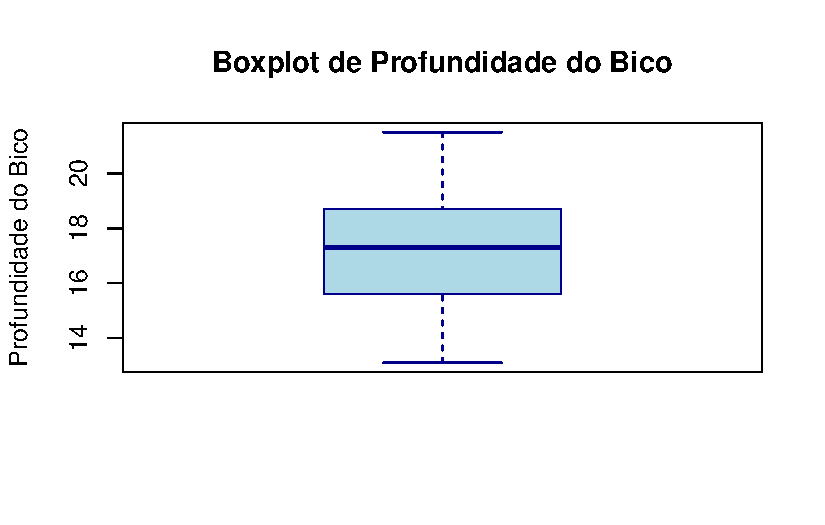
\includegraphics{r_files/figure-pdf/unnamed-chunk-2-1.pdf}

Analisando esse gráfico de dispersão existe a divisão da população de
pinguins em dois grupos, um quando o comprimento da nadadeira é menor a
profundidade do bico é maior e outro quando o comprimento da nadadeira é
maior a profundidade do bico é menor, ou seja, o coeficiente de
correlação linear \textbf{r} será negativo

\begin{Shaded}
\begin{Highlighting}[]
\FunctionTok{plot}\NormalTok{(profundidade\_bico }\SpecialCharTok{\textasciitilde{}}\NormalTok{ comprimento\_bico, }\AttributeTok{data =}\NormalTok{ dados\_clean, }
        \AttributeTok{main =} \StringTok{"Profundidade do Bico por Comprimento Bico"}\NormalTok{,}
        \AttributeTok{xlab =} \StringTok{"comprimento\_bico"}\NormalTok{, }\AttributeTok{ylab =} \StringTok{"Profundidade Bico"}\NormalTok{)}
\end{Highlighting}
\end{Shaded}

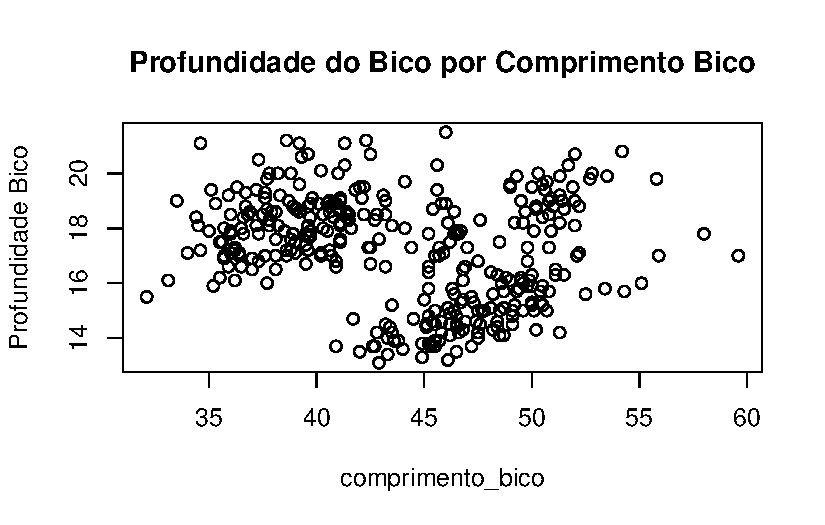
\includegraphics{r_files/figure-pdf/unnamed-chunk-3-1.pdf}

O gráfico de dispersão com a variável \textbf{comprimento\_bico}, não é
possível encontrar alguma relação entre as variáveis.

\begin{Shaded}
\begin{Highlighting}[]
\FunctionTok{plot}\NormalTok{(profundidade\_bico }\SpecialCharTok{\textasciitilde{}}\NormalTok{ massa\_corporal, }\AttributeTok{data =}\NormalTok{ dados\_clean, }
        \AttributeTok{main =} \StringTok{"Profundidade do Bico por Massa Corporal"}\NormalTok{,}
        \AttributeTok{xlab =} \StringTok{"massa\_corporal"}\NormalTok{, }\AttributeTok{ylab =} \StringTok{"Profundidade Bico"}\NormalTok{)}
\end{Highlighting}
\end{Shaded}

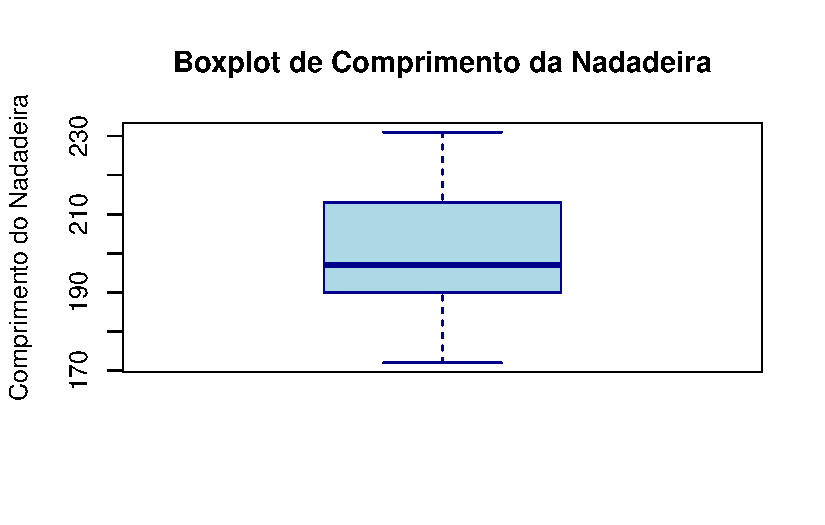
\includegraphics{r_files/figure-pdf/unnamed-chunk-4-1.pdf}

Com relação à \textbf{massa\_corporal} é possível observar que quanto
maior a massa corporal menor a profundidade do bico e quando menor a
massa corporal maior será o bico, logo, o coeficiente de correlação
linear também será negativo

\begin{Shaded}
\begin{Highlighting}[]
\FunctionTok{library}\NormalTok{(GGally)}
\end{Highlighting}
\end{Shaded}

\begin{verbatim}
Carregando pacotes exigidos: ggplot2
\end{verbatim}

\begin{verbatim}
Registered S3 method overwritten by 'GGally':
  method from   
  +.gg   ggplot2
\end{verbatim}

\begin{Shaded}
\begin{Highlighting}[]
\NormalTok{graf1 }\OtherTok{\textless{}{-}} \FunctionTok{ggpairs}\NormalTok{(dados\_clean, }\AttributeTok{columns =} \DecValTok{3}\SpecialCharTok{:}\DecValTok{6}\NormalTok{, ggplot2}\SpecialCharTok{::}\FunctionTok{aes}\NormalTok{(}\AttributeTok{colour=}\NormalTok{especie))}
\NormalTok{graf1}
\end{Highlighting}
\end{Shaded}

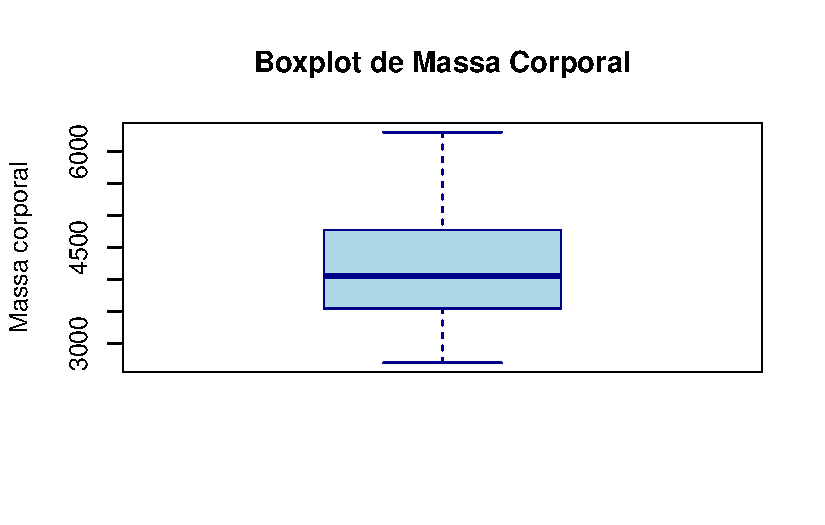
\includegraphics{r_files/figure-pdf/unnamed-chunk-5-1.pdf}

Importante ressaltar que as variáveis preditoras comprimento nadadeira e
massa corporal podem ocasionar uma multicolinearidade, pois o
coeficiente de correlação linear (Corr) é maior do que 0.8. Dessa forma,
esse fato tem que ser corrigido no nosso modelo a ser escolhido.

\section{3. Modelos}\label{modelos}

Inicialmente temos o primeiro modelo

\begin{Shaded}
\begin{Highlighting}[]
\NormalTok{modelo1 }\OtherTok{\textless{}{-}} \FunctionTok{lm}\NormalTok{(profundidade\_bico }\SpecialCharTok{\textasciitilde{}}\NormalTok{ . }\SpecialCharTok{{-}}\NormalTok{especie, }\AttributeTok{data =}\NormalTok{ dados\_clean)}
\FunctionTok{summary}\NormalTok{(modelo1)}
\end{Highlighting}
\end{Shaded}

\begin{verbatim}

Call:
lm(formula = profundidade_bico ~ . - especie, data = dados_clean)

Residuals:
    Min      1Q  Median      3Q     Max 
-2.7329 -0.7450 -0.1286  0.6913  4.4479 

Coefficients:
                        Estimate Std. Error t value Pr(>|t|)    
(Intercept)           -1.124e+02  1.550e+02  -0.725  0.46888    
ilhaDream              1.032e+00  1.849e-01   5.584 4.97e-08 ***
ilhaTorgersen          1.127e+00  2.150e-01   5.239 2.91e-07 ***
comprimento_bico       9.445e-03  1.680e-02   0.562  0.57446    
comprimento_nadadeira -5.480e-02  1.057e-02  -5.184 3.82e-07 ***
massa_corporal        -5.304e-04  1.885e-04  -2.814  0.00518 ** 
sexomacho              2.194e+00  1.486e-01  14.766  < 2e-16 ***
ano                    7.010e-02  7.738e-02   0.906  0.36567    
---
Signif. codes:  0 '***' 0.001 '**' 0.01 '*' 0.05 '.' 0.1 ' ' 1

Residual standard error: 1.095 on 325 degrees of freedom
Multiple R-squared:  0.697, Adjusted R-squared:  0.6905 
F-statistic: 106.8 on 7 and 325 DF,  p-value: < 2.2e-16
\end{verbatim}

Devido a existência de uma correlação da variável resposta
\textbf{profundidade\_bico} com as variáveis explicativas
\textbf{comprimento\_nadadeira} e \textbf{massa\_corporal} como já foi
observado anteriormente elas variam em sentidos opostos, no entanto
essas variáveis preditoras podem ocasionar a multicolinearidade. Assim,
analisando o modelo 1 não existe nenhuma anormalidade com as
estimativas, pois a medida que aumenta uma unidade no comprimento da
nadadeira, tem uma estimativa de diminuir a profundidade do bico em
-5.480e-02 o mesmo acontece com a massa corporal, pois quando aumenta
uma unidade na massa corporal tem a estimativa de diminuir a
profundidade do bico em -5.304e-04.

No entanto, a variável preditora \textbf{comprimento\_bico} possui o
valor P igual a 0.57446 o que é maior do que 10\%, sendo uma boa
alternativa retirá-la do modelo 1.

\begin{Shaded}
\begin{Highlighting}[]
\NormalTok{modelo2 }\OtherTok{\textless{}{-}} \FunctionTok{update}\NormalTok{(modelo1, }\SpecialCharTok{\textasciitilde{}}\NormalTok{ . }\SpecialCharTok{{-}}\NormalTok{comprimento\_bico)}
\FunctionTok{summary}\NormalTok{(modelo2)}
\end{Highlighting}
\end{Shaded}

\begin{verbatim}

Call:
lm(formula = profundidade_bico ~ ilha + comprimento_nadadeira + 
    massa_corporal + sexo + ano, data = dados_clean)

Residuals:
    Min      1Q  Median      3Q     Max 
-2.7533 -0.7624 -0.1015  0.7184  4.4564 

Coefficients:
                        Estimate Std. Error t value Pr(>|t|)    
(Intercept)           -1.051e+02  1.543e+02  -0.681  0.49635    
ilhaDream              1.069e+00  1.728e-01   6.185 1.86e-09 ***
ilhaTorgersen          1.119e+00  2.144e-01   5.219 3.20e-07 ***
comprimento_nadadeira -5.223e-02  9.519e-03  -5.486 8.25e-08 ***
massa_corporal        -5.259e-04  1.881e-04  -2.796  0.00548 ** 
sexomacho              2.208e+00  1.463e-01  15.090  < 2e-16 ***
ano                    6.638e-02  7.701e-02   0.862  0.38938    
---
Signif. codes:  0 '***' 0.001 '**' 0.01 '*' 0.05 '.' 0.1 ' ' 1

Residual standard error: 1.094 on 326 degrees of freedom
Multiple R-squared:  0.6968,    Adjusted R-squared:  0.6912 
F-statistic: 124.8 on 6 and 326 DF,  p-value: < 2.2e-16
\end{verbatim}

Com o novo modelo o valor R-squared obteve um aumento de 0.0007,
indicando que o modelo 2 é melhor do que o modelo 1, pelo fato do valor
R\^{}2 ser maior. No entanto, é possível realizar uma melhoria nesse
modelo pelo fato da variável preditora ano possuir um valor P superior a
10\%

\begin{Shaded}
\begin{Highlighting}[]
\NormalTok{modelo3 }\OtherTok{\textless{}{-}} \FunctionTok{update}\NormalTok{(modelo2, }\SpecialCharTok{\textasciitilde{}}\NormalTok{ . }\SpecialCharTok{{-}}\NormalTok{ano)}
\FunctionTok{summary}\NormalTok{(modelo3)}
\end{Highlighting}
\end{Shaded}

\begin{verbatim}

Call:
lm(formula = profundidade_bico ~ ilha + comprimento_nadadeira + 
    massa_corporal + sexo, data = dados_clean)

Residuals:
    Min      1Q  Median      3Q     Max 
-2.6861 -0.7580 -0.0936  0.6901  4.5334 

Coefficients:
                        Estimate Std. Error t value Pr(>|t|)    
(Intercept)           27.9043913  1.3521204  20.638  < 2e-16 ***
ilhaDream              1.0626246  0.1726214   6.156 2.19e-09 ***
ilhaTorgersen          1.1179289  0.2142790   5.217 3.23e-07 ***
comprimento_nadadeira -0.0499521  0.0091429  -5.464 9.26e-08 ***
massa_corporal        -0.0005633  0.0001829  -3.079  0.00225 ** 
sexomacho              2.2176123  0.1458956  15.200  < 2e-16 ***
---
Signif. codes:  0 '***' 0.001 '**' 0.01 '*' 0.05 '.' 0.1 ' ' 1

Residual standard error: 1.094 on 327 degrees of freedom
Multiple R-squared:  0.6961,    Adjusted R-squared:  0.6914 
F-statistic: 149.8 on 5 and 327 DF,  p-value: < 2.2e-16
\end{verbatim}

Logo, podemos perceber uma melhoria nos valores tanto na estimativa,
como também no valor R\^{}2,~ 0.6914, aumentando 0.0002, o que indica
que houve uma melhora no modelo.Para confirmar essa ideia vamos calcular
a medida AIC dos modelos.

\section{4. Métodos de seleção de
modelos}\label{muxe9todos-de-seleuxe7uxe3o-de-modelos}

\subsection{4.1 Medida AIC}\label{medida-aic}

Tendo em vista que temos três possíveis modelos calculamos o AIC

\begin{Shaded}
\begin{Highlighting}[]
\FunctionTok{AIC}\NormalTok{(modelo1)}
\end{Highlighting}
\end{Shaded}

\begin{verbatim}
[1] 1015.66
\end{verbatim}

\begin{Shaded}
\begin{Highlighting}[]
\FunctionTok{AIC}\NormalTok{(modelo2)}
\end{Highlighting}
\end{Shaded}

\begin{verbatim}
[1] 1013.983
\end{verbatim}

\begin{Shaded}
\begin{Highlighting}[]
\FunctionTok{AIC}\NormalTok{(modelo3)}
\end{Highlighting}
\end{Shaded}

\begin{verbatim}
[1] 1012.741
\end{verbatim}

Dessa forma, o menor valor AIC indica o melhor modelo que no caso seria
o modelo 3

\subsection{4.2 Medida BIC}\label{medida-bic}

Agora vamos calcular o melhor modelo possível segundo o BIC

\begin{Shaded}
\begin{Highlighting}[]
\FunctionTok{BIC}\NormalTok{(modelo1)}
\end{Highlighting}
\end{Shaded}

\begin{verbatim}
[1] 1049.933
\end{verbatim}

\begin{Shaded}
\begin{Highlighting}[]
\FunctionTok{BIC}\NormalTok{(modelo2)}
\end{Highlighting}
\end{Shaded}

\begin{verbatim}
[1] 1044.448
\end{verbatim}

\begin{Shaded}
\begin{Highlighting}[]
\FunctionTok{BIC}\NormalTok{(modelo3)}
\end{Highlighting}
\end{Shaded}

\begin{verbatim}
[1] 1039.398
\end{verbatim}

Assim, o menor valor BIC indica o melhor modelo que no caso seria o
modelo 3, faz-se o BIC para possuir uma melhor confirmação sobre qual é
o caminho preferível.

\subsection{4.3 Comparação de modelos
encaixados(ANOVA)}\label{comparauxe7uxe3o-de-modelos-encaixadosanova}

Comparação de modelos aninhados, ou seja, quando um ou mais modelo é
obtido como sub-conjunto do(s) outro(s)

\begin{Shaded}
\begin{Highlighting}[]
\FunctionTok{anova}\NormalTok{(modelo1,modelo2)}
\end{Highlighting}
\end{Shaded}

\begin{verbatim}
Analysis of Variance Table

Model 1: profundidade_bico ~ (especie + ilha + comprimento_bico + comprimento_nadadeira + 
    massa_corporal + sexo + ano) - especie
Model 2: profundidade_bico ~ ilha + comprimento_nadadeira + massa_corporal + 
    sexo + ano
  Res.Df    RSS Df Sum of Sq      F Pr(>F)
1    325 390.04                           
2    326 390.42 -1  -0.37913 0.3159 0.5745
\end{verbatim}

Como o p-valor (0.5745) é significativamente maior que 0.05, não há
evidências suficientes para concluir que a remoção da variável
comprimento\_bico melhora o modelo de forma significativa. Portanto, a
inclusão do comprimento do bico é justificada, pois a exclusão dessa
variável não resulta em um modelo que explique melhor a variação na
profundidade do bico. Em resumo, a análise sugere que o comprimento do
bico deve ser mantido no modelo para melhor entendimento dos fatores que
influenciam a profundidade do bico.

\begin{Shaded}
\begin{Highlighting}[]
\FunctionTok{anova}\NormalTok{(modelo2,modelo3)}
\end{Highlighting}
\end{Shaded}

\begin{verbatim}
Analysis of Variance Table

Model 1: profundidade_bico ~ ilha + comprimento_nadadeira + massa_corporal + 
    sexo + ano
Model 2: profundidade_bico ~ ilha + comprimento_nadadeira + massa_corporal + 
    sexo
  Res.Df    RSS Df Sum of Sq      F Pr(>F)
1    326 390.42                           
2    327 391.31 -1  -0.88963 0.7428 0.3894
\end{verbatim}

Como o p-valor (0.3894) é significativamente maior que 0.05, não há
evidências suficientes para concluir que a remoção da variável ano
melhora o modelo de forma significativa. Assim, a inclusão do ano no
Modelo 1 é justificada, pois a exclusão dessa variável não resulta em um
modelo que explique melhor a variação na profundidade do bico. Em
resumo, os dados sugerem que a variável ano desempenha um papel
importante na modelagem da profundidade do bico, e sua remoção não é
recomendada.

\begin{Shaded}
\begin{Highlighting}[]
\FunctionTok{anova}\NormalTok{(modelo1,modelo3)}
\end{Highlighting}
\end{Shaded}

\begin{verbatim}
Analysis of Variance Table

Model 1: profundidade_bico ~ (especie + ilha + comprimento_bico + comprimento_nadadeira + 
    massa_corporal + sexo + ano) - especie
Model 2: profundidade_bico ~ ilha + comprimento_nadadeira + massa_corporal + 
    sexo
  Res.Df    RSS Df Sum of Sq      F Pr(>F)
1    325 390.04                           
2    327 391.31 -2   -1.2688 0.5286 0.5899
\end{verbatim}

Dado que o p-valor (0.5899) é significativamente maior que 0.05, não há
evidências suficientes para afirmar que a remoção das variáveis
comprimento do bico, ilha, comprimento da nadadeira, massa corporal e
sexo (considerando a comparação com o Modelo 1) resulta em um modelo
significativamente melhor. Isso sugere que a inclusão das variáveis do
Modelo 1 é justificada, pois a exclusão de qualquer uma delas não
melhora a explicação da variação na profundidade do bico.

Em síntese, os resultados indicam que as variáveis incluídas no Modelo 1
desempenham papéis importantes e devem ser mantidas para uma modelagem
adequada da profundidade do bico.

\section{5. Modelo selecionado(modelo
3)}\label{modelo-selecionadomodelo-3}

Levando em consideração os métodos de seleção de um modelo, podemos
verificar que para realizar previsões e também interpretações o modelo a
ser adotado é o modelo 3.

\begin{Shaded}
\begin{Highlighting}[]
\FunctionTok{plot}\NormalTok{(modelo3)}
\end{Highlighting}
\end{Shaded}

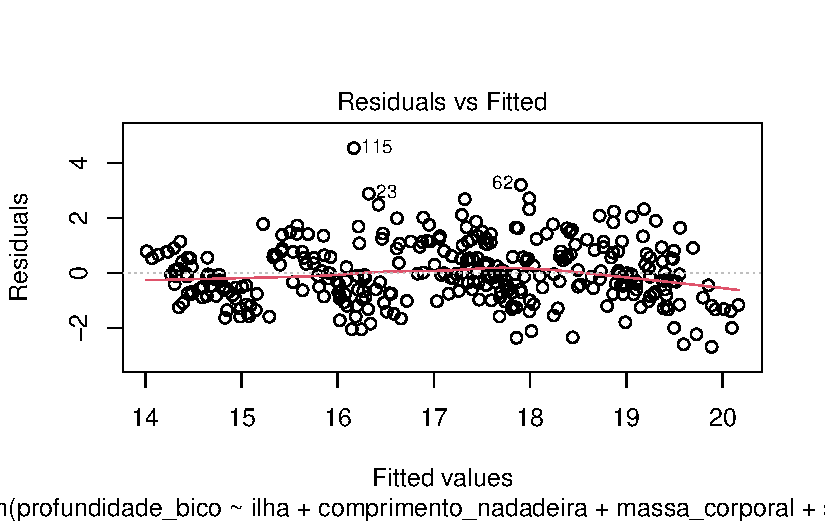
\includegraphics{r_files/figure-pdf/unnamed-chunk-14-1.pdf}

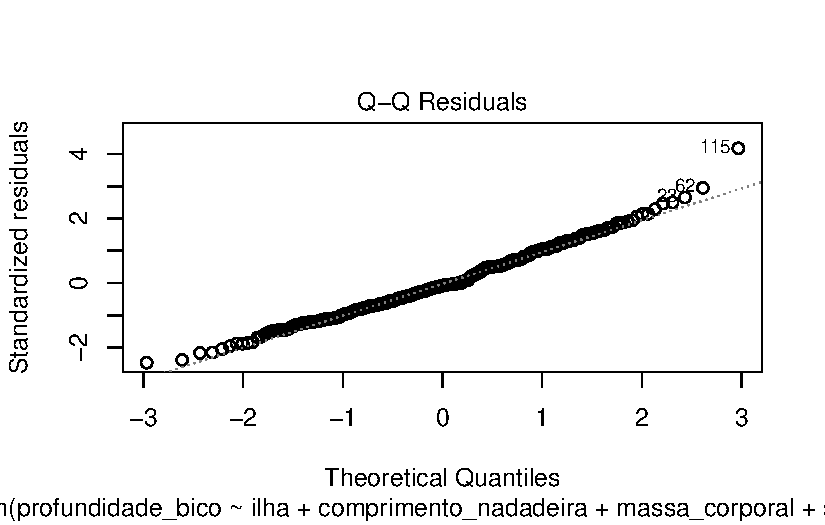
\includegraphics{r_files/figure-pdf/unnamed-chunk-14-2.pdf}

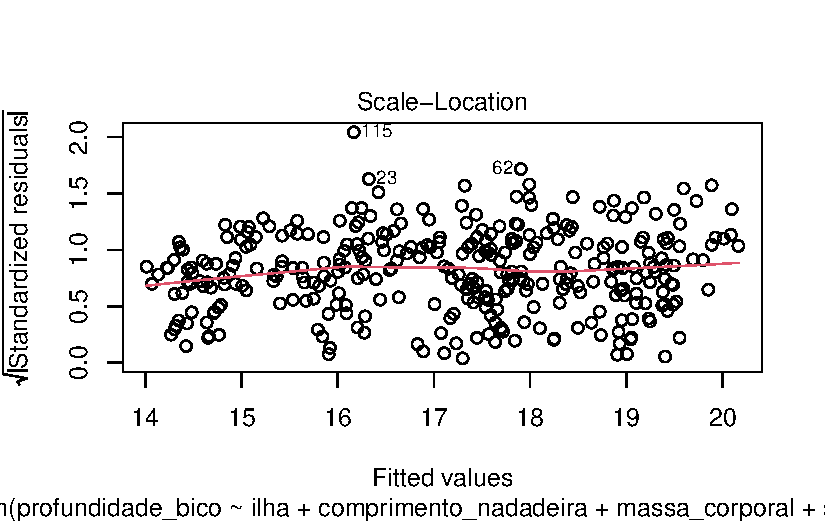
\includegraphics{r_files/figure-pdf/unnamed-chunk-14-3.pdf}

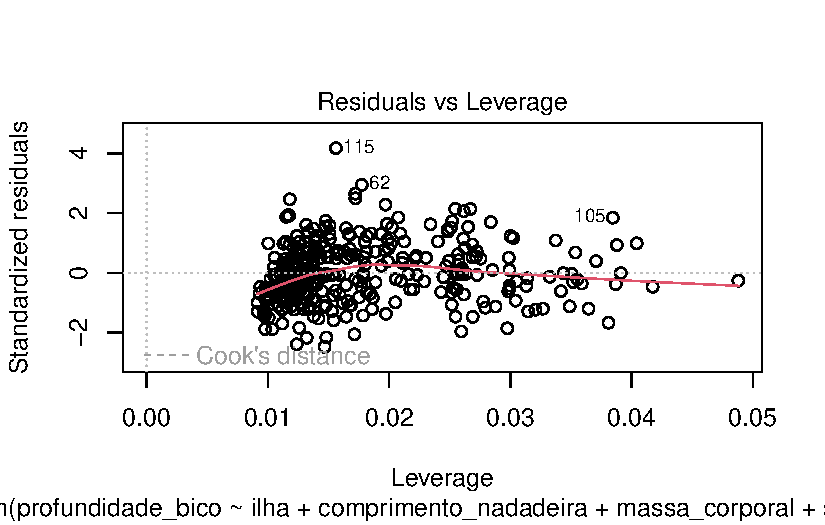
\includegraphics{r_files/figure-pdf/unnamed-chunk-14-4.pdf}

\subsection{5.1 Cometários}\label{cometuxe1rios}

\begin{itemize}
\item
  \textbf{Residuals vs Fitted:} Os pontos estão distribuídos de forma
  aleatória, sem nenhum padrão específico na forma de U ou V, logo,
  verificando a linearidade e a homocedasticidade.
\item
  \textbf{Normal Q-Q}: Os pontos seguem a linha reta, ajudando a
  suposição de que os resíduos seguem uma distribuição normal.
\item
  \textbf{Scale-Location (ou Spread-Location)}: Os pontos estão
  espalhados em torno de uma linha horizontal, verificando verificando a
  homocedasticidade.
\item
  \textbf{Residuals vs Leverage}: esse gráfico ajuda a identificar
  outliers e pontos com alta alavancagem
\end{itemize}

\section{6. Interpretação do modelo
selecionado}\label{interpretauxe7uxe3o-do-modelo-selecionado}

\begin{Shaded}
\begin{Highlighting}[]
\CommentTok{\#install.packages("report")}

\FunctionTok{library}\NormalTok{(report)}

\FunctionTok{report}\NormalTok{(modelo3)}
\end{Highlighting}
\end{Shaded}

\begin{verbatim}
We fitted a linear model (estimated using OLS) to predict profundidade_bico
with ilha, comprimento_nadadeira, massa_corporal and sexo (formula:
profundidade_bico ~ ilha + comprimento_nadadeira + massa_corporal + sexo). The
model explains a statistically significant and substantial proportion of
variance (R2 = 0.70, F(5, 327) = 149.78, p < .001, adj. R2 = 0.69). The model's
intercept, corresponding to ilha = Biscoe, comprimento_nadadeira = 0,
massa_corporal = 0 and sexo = fêmea, is at 27.90 (95% CI [25.24, 30.56], t(327)
= 20.64, p < .001). Within this model:

  - The effect of ilha [Dream] is statistically significant and positive (beta =
1.06, 95% CI [0.72, 1.40], t(327) = 6.16, p < .001; Std. beta = 0.54, 95% CI
[0.37, 0.71])
  - The effect of ilha [Torgersen] is statistically significant and positive
(beta = 1.12, 95% CI [0.70, 1.54], t(327) = 5.22, p < .001; Std. beta = 0.57,
95% CI [0.35, 0.78])
  - The effect of comprimento nadadeira is statistically significant and negative
(beta = -0.05, 95% CI [-0.07, -0.03], t(327) = -5.46, p < .001; Std. beta =
-0.36, 95% CI [-0.48, -0.23])
  - The effect of massa corporal is statistically significant and negative (beta
= -5.63e-04, 95% CI [-9.23e-04, -2.03e-04], t(327) = -3.08, p = 0.002; Std.
beta = -0.23, 95% CI [-0.38, -0.08])
  - The effect of sexo [macho] is statistically significant and positive (beta =
2.22, 95% CI [1.93, 2.50], t(327) = 15.20, p < .001; Std. beta = 1.13, 95% CI
[0.98, 1.27])

Standardized parameters were obtained by fitting the model on a standardized
version of the dataset. 95% Confidence Intervals (CIs) and p-values were
computed using a Wald t-distribution approximation.
\end{verbatim}

(R² = 0,70; F(5, 327) = 149,78; p \textless{} 0,001; R² ajustado =
0,69). Em termos simples, isso significa que \textbf{70\%} da variação
observada na profundidade do bico pode ser explicada pelas variáveis
incluídas no modelo. Esse valor indica um bom ajuste do modelo.

O intercepto do modelo, que corresponde à \textbf{profundidade do bico}
quando, ilha = Biscoe, comprimento\_nadadeira = 0, massa\_corporal = 0,
sexo = fêmea, é estimado em 27,90 mm, com um intervalo de confiança de
95\% {[}25,24, 30,56{]}. O valor t associado ao intercepto é 20,64 (p
\textless{} 0,001), o que indica que ele é estatisticamente
significativo.

O efeito de estar na \textbf{ilha Dream} é positivo e estatisticamente
significativo. Isso significa que, em média, os indivíduos nessa ilha
têm uma profundidade de bico 1,06 mm maior do que os da ilha Biscoe, com
um intervalo de confiança de 95\% entre {[}0,72, 1,40{]} (t(327) = 6,16,
p \textless{} 0,001). O coeficiente padronizado (beta padronizado) é
0,54, o que sugere que esse efeito é moderadamente forte em relação às
outras variáveis do modelo.

Estar na \textbf{ilha Torgersen} também tem um efeito positivo
significativo, resultando, em média, numa profundidade de bico 1,12 mm
maior do que na ilha Biscoe (IC 95\% {[}0,70, 1,54{]}; t(327) = 5,22, p
\textless{} 0,001). O coeficiente padronizado é 0,57, indicando que o
efeito da ilha Torgersen é ligeiramente mais forte que o da ilha Dream.

O efeito do \textbf{comprimento da nadadeira} é negativo e
estatisticamente significativo. Cada aumento de uma unidade no
comprimento da nadadeira está associado a uma redução de 0,05 mm na
profundidade do bico (IC 95\% {[}-0,07, -0,03{]}; t(327) = -5,46, p
\textless{} 0,001). O coeficiente padronizado é -0,36, o que sugere um
efeito moderado e inverso --- quanto maior a nadadeira, menor a
profundidade do bico.

O efeito da \textbf{massa corporal} também é negativo e significativo.
Cada incremento na massa corporal está associado a uma redução de
0,000563 mm na profundidade do bico (IC 95\% {[}-0,000923, -0,000203{]};
t(327) = -3,08, p = 0,002). Embora esse efeito seja pequeno, ele é
estatisticamente significativo e o coeficiente padronizado (-0,23)
sugere que seu impacto relativo é menor em comparação com as outras
variáveis.

Ser do \textbf{sexo masculino} tem um efeito positivo \textbf{muito
forte} na profundidade do bico. Machos tendem a ter, em média, 2,22 mm a
mais de profundidade de bico do que fêmeas (IC 95\% {[}1,93, 2,50{]};
t(327) = 15,20, p \textless{} 0,001). O coeficiente padronizado é 1,13,
indicando que o sexo é a variável com o efeito mais forte no modelo.

Logo podemos concluir que os pinguins das ilhas Dream e Torgersen têm
bicos mais profundos do que a ilha Biscoe, o comprimento da nadadeira e
a massa corporal estão inversamente associados à profundidade do bico, e
por fim machos tendem a ter bicos sifnificamente mais profundos que as
fêmeas, o que pode ter implicações para estudos comportamentais ou
ecológicos.

\subsection{6.1 Coeficientes
padronizados}\label{coeficientes-padronizados}

\begin{Shaded}
\begin{Highlighting}[]
\CommentTok{\#install.packages("lm.beta")}

\NormalTok{lm.beta}\SpecialCharTok{::}\FunctionTok{lm.beta}\NormalTok{(modelo2)}
\end{Highlighting}
\end{Shaded}

\begin{verbatim}

Call:
lm(formula = profundidade_bico ~ ilha + comprimento_nadadeira + 
    massa_corporal + sexo + ano, data = dados_clean)

Standardized Coefficients::
          (Intercept)             ilhaDream         ilhaTorgersen 
                   NA             0.2623994             0.1981176 
comprimento_nadadeira        massa_corporal             sexomacho 
           -0.3717084            -0.2150356             0.5615308 
                  ano 
            0.0274019 
\end{verbatim}

\section{7. Previsões}\label{previsuxf5es}

Resumo sobre os dados observados:

\begin{Shaded}
\begin{Highlighting}[]
\FunctionTok{summary}\NormalTok{(dados)}
\end{Highlighting}
\end{Shaded}

\begin{verbatim}
       X            especie              ilha           comprimento_bico
 Min.   :  1.00   Length:344         Length:344         Min.   :32.10   
 1st Qu.: 86.75   Class :character   Class :character   1st Qu.:39.23   
 Median :172.50   Mode  :character   Mode  :character   Median :44.45   
 Mean   :172.50                                         Mean   :43.92   
 3rd Qu.:258.25                                         3rd Qu.:48.50   
 Max.   :344.00                                         Max.   :59.60   
                                                        NA's   :2       
 profundidade_bico comprimento_nadadeira massa_corporal     sexo          
 Min.   :13.10     Min.   :172.0         Min.   :2700   Length:344        
 1st Qu.:15.60     1st Qu.:190.0         1st Qu.:3550   Class :character  
 Median :17.30     Median :197.0         Median :4050   Mode  :character  
 Mean   :17.15     Mean   :200.9         Mean   :4202                     
 3rd Qu.:18.70     3rd Qu.:213.0         3rd Qu.:4750                     
 Max.   :21.50     Max.   :231.0         Max.   :6300                     
 NA's   :2         NA's   :2             NA's   :2                        
      ano      
 Min.   :2007  
 1st Qu.:2007  
 Median :2008  
 Mean   :2008  
 3rd Qu.:2009  
 Max.   :2009  
               
\end{verbatim}




\end{document}
